\section{HSR's Software and External Devices}
% In this section briefly describe the software and hardware of the robot

\setlength\intextsep{0pt}
\begin{wrapfigure}[12]{RH}{0.3\textwidth}
	\centering
	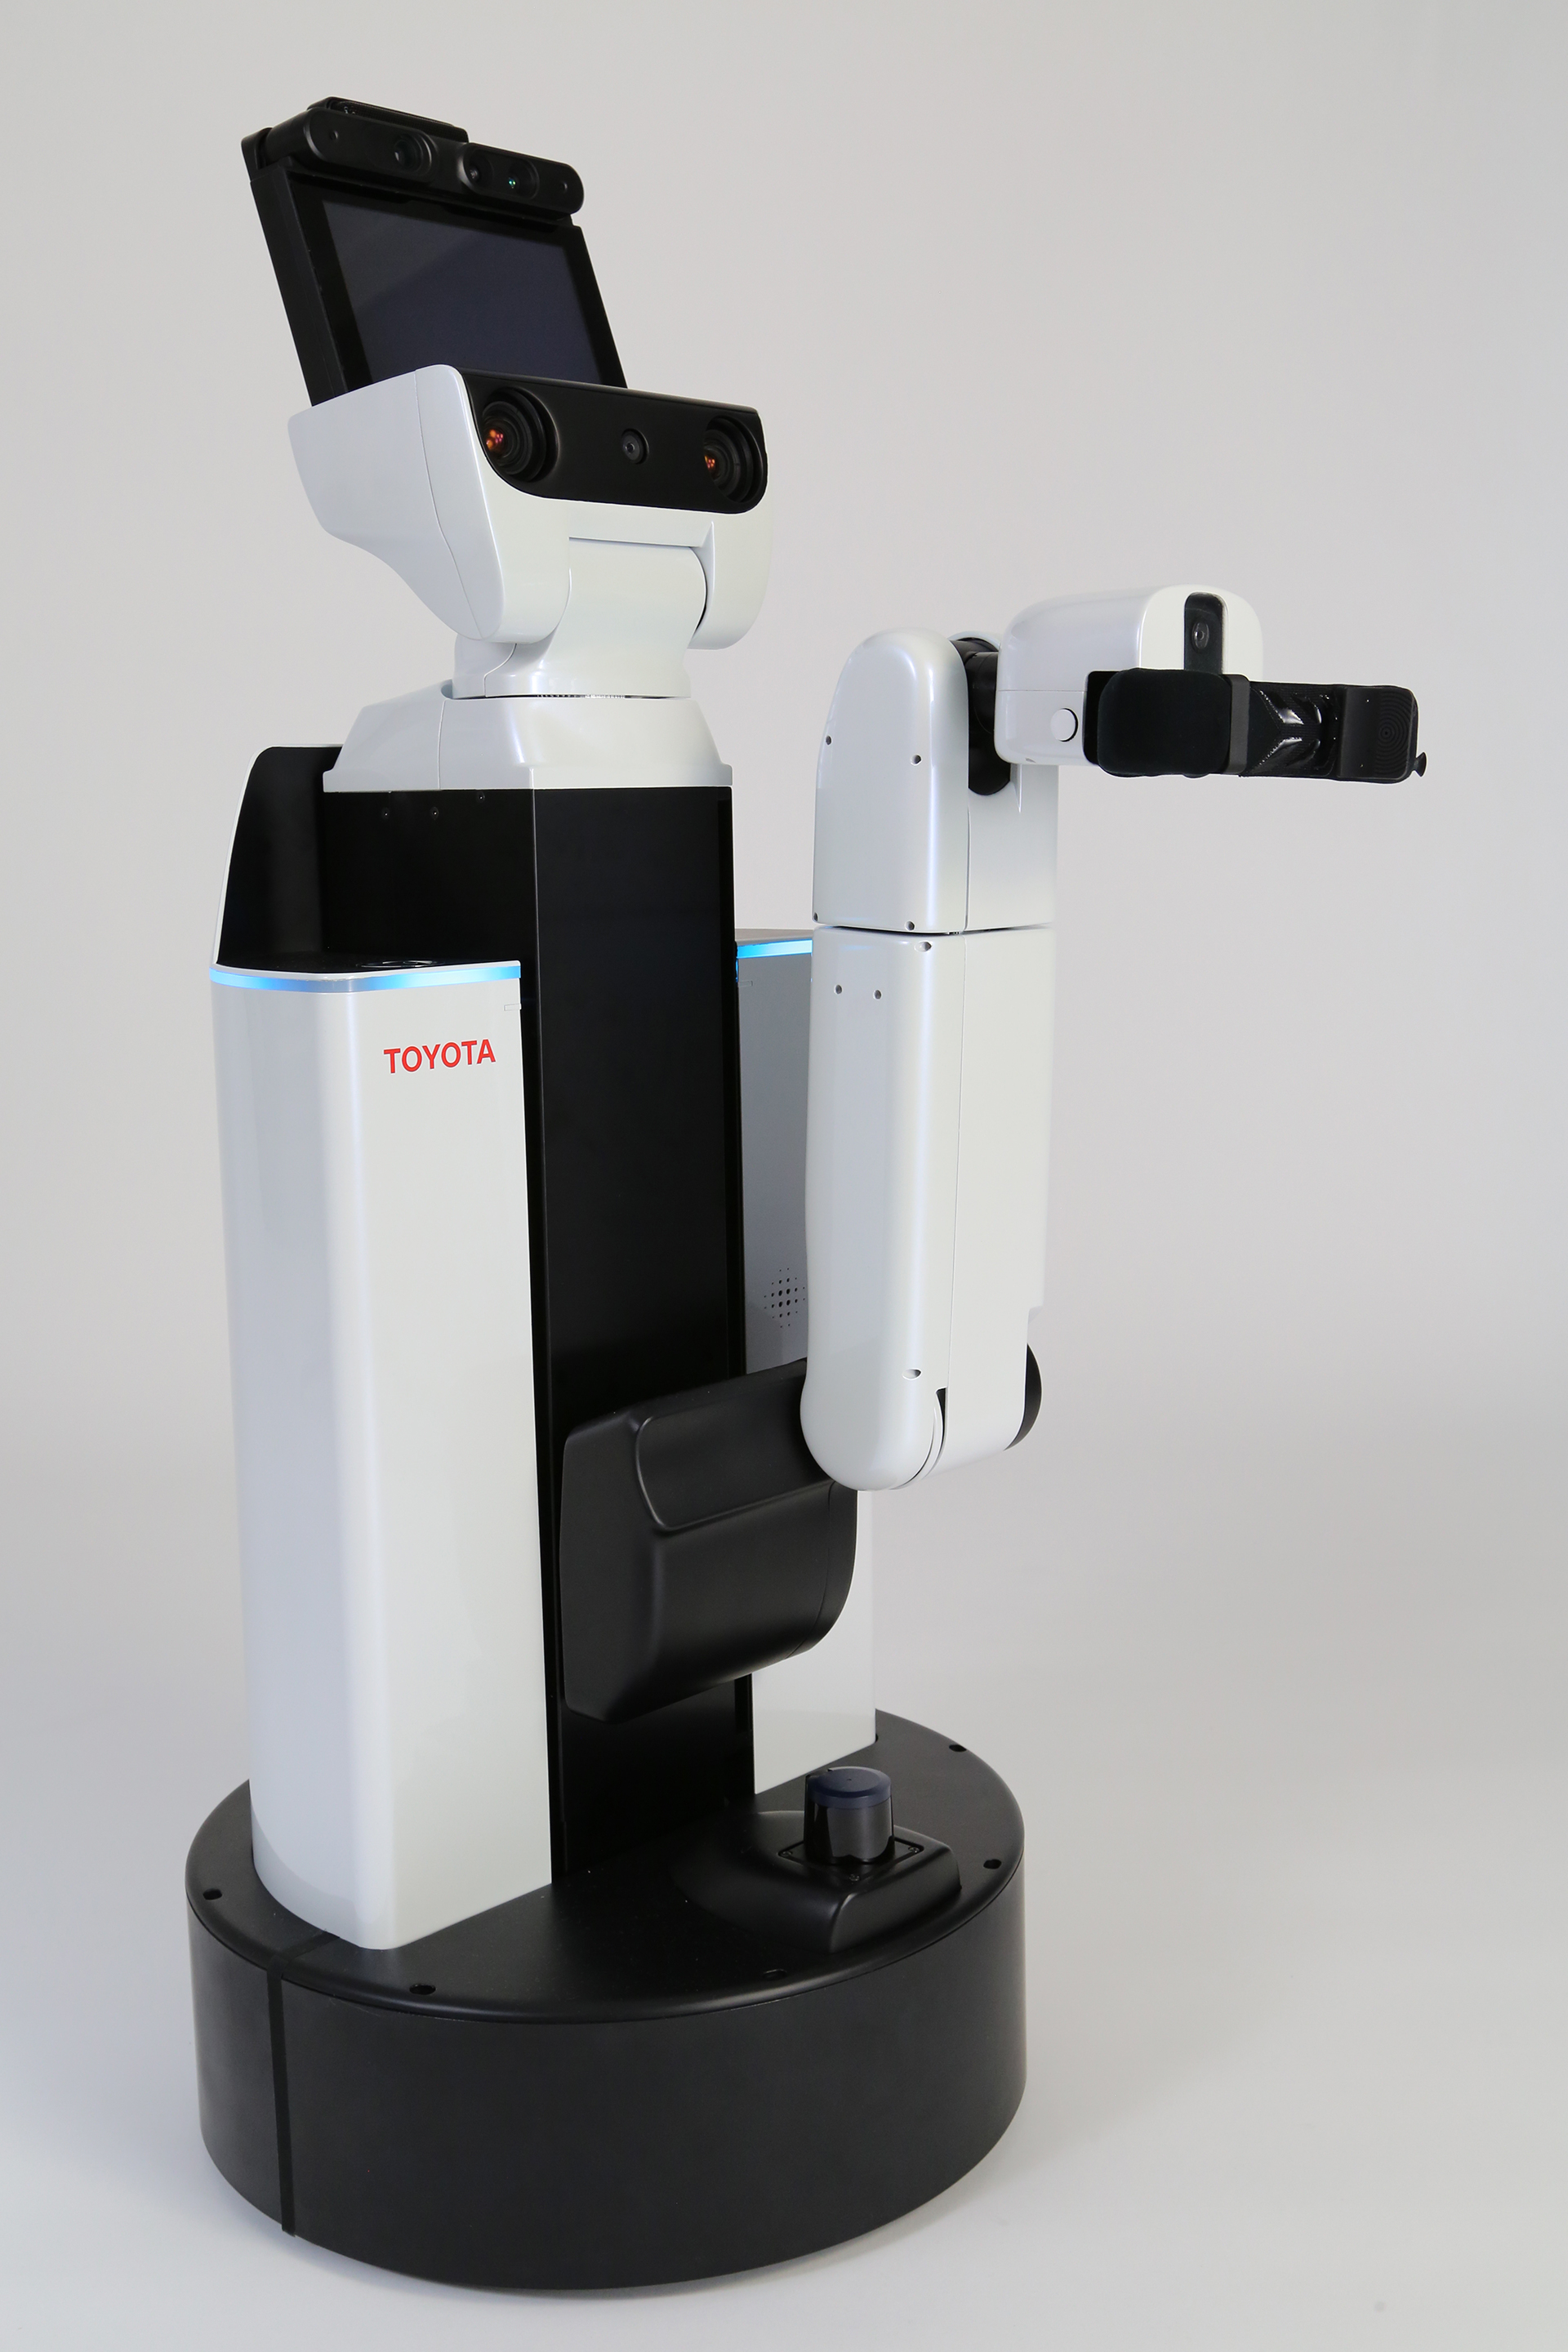
\includegraphics[width=0.3\textwidth]{Figures/Toyota_HSR}
	\caption{The Toyota\texttrademark\hspace{0em} HSR Robot, HERO}
	\label{fig:hsr}
\end{wrapfigure}

We use a standard Toyota\texttrademark\hspace{0em} HSR robot. To differentiate our unit, we named it HERO. We wanted to link it's name to our AMIGO and SERGIO domestic service robots.

\subsubsection{HERO's Software Description}
% Please describe in this section the software you are using to control your robot. Consider the following example:

An overview of the software used by the Tech United Eindhoven @Home robots can be found in Table~\ref{tab:softwarespec}.
All our software is developed open-source at GitHub\footnote{\url{https://github.com/tue-robotics}}.
\\\newline
%Currently, we have some \emph{image\_recognition} packages released into the current ROS Kinetic distribution and can be installed with use of \textit{apt}.
\vspace{0.8cm}
\begin{table}[h]
    \begin{center}
    \caption{Software overview}
    \label{tab:softwarespec}
    %\vspace{-0.1cm}
    \renewcommand{\arraystretch}{1.0}
    \setlength{\tabcolsep}{5pt}
        \begin{tabular}{p{0.3\textwidth} p{0.7\textwidth}}
            \toprule
            Operating system & Ubuntu 16.04 LTS Server\\

            Middleware & ROS Kinetic~\cite{Quigley2009}\\

%            Low-level control software & Orocos Real-Time Toolkit~\cite{Bruyninckx2001}\newline
%            \url{https://github.com/tue-robotics/rtt_control_components}
%            \\

            Simulation & Gazebo\\

            World model & \acrfull{ed}, custom \newline
            \url{https://github.com/tue-robotics/ed}\\

            Localization & Monte Carlo~\cite{Fox2003} using \gls{ed}, custom \newline \url{https://github.com/tue-robotics/ed_localization}\\

            SLAM & Gmapping\\

            Navigation & CB Base navigation
            \newline
            \url{https://github.com/tue-robotics/cb_base_navigation}
            \newline
            Global: custom A* planner\newline Local: modified ROS DWA~\cite{Fox1997}\\

            Arm navigation & MoveIt!\\

            Object recognition & image\_recognition\_tensorflow \newline
			\url{https://github.com/tue-robotics/image_recognition/tree/master/image_recognition_openface}\\

            People detection & Custom implementation using contour matching \newline
            \url{https://github.com/tue-robotics/ed_perception}
            \\
            Face detection \& recognition & image\_recognition\_openface \newline \url{https://github.com/tue-robotics/image_recognition/tree/master/image_recognition_openface} \\

            Speech recognition & Julius Speech Recognition \newline
            \url{https://github.com/julius-speech/julius}\\
            Speech synthesis & Toyota\texttrademark \hspace{0em} Text-to-Speech\\
            Task executors & SMACH \newline
            \url{https://github.com/tue-robotics/tue_robocup}\\
            \bottomrule
        \end{tabular}
    \end{center}
\end{table}

This is our current software implementation, which matches our own robots, AMIGO and SERGIO, which have participated with in the open platform league.

\subsubsection{External Devices}
% Please describe in this section the external devices used by your robot. Consider the following example:

\textit{HERO relies on the following external hardware:}

\begin{itemize}
    \item Official Standard Laptop
\end{itemize}

\subsubsection{Cloud Services}
% Please describe in this section the Cloud Services and online software used by your robot. Consider the following example:

\textit{HERO connects the following cloud services:} None
%\begin{itemize}
%	\item Localization and mapping: Geolocalization system.
%	\item Navigation: Navigator
%	\item Speech recognition: All-purpose recognizer.
%\end{itemize}
